\section*{Цель работы.}
Изучение работы с файдами в математическом пакете MatLab.

\newcommand{\exOne}{Реализовать функцию, которая будет брать исходные данные из файла в соответствии с таблицей 1. Исходные данные данной таблицы должны включать диапазон и количество точек для каждой переменной.}
\newcommand{\exTwo}{Реализовать функцию, которая будет брать исходные данные из файла в соответствии с таблицей 2. Исходные данные данной таблицы должны включать диапазон, количество точек и вариативность \textit{semilogx}, \textit{semilogx}, \textit{loglog}, \textit{plot}.}
\newcommand{\exThree}{Реализовать алгоритм, который будет в соответствии с прототипом из таблицы 5 записывать результат работы функции из задания 1 в файл.}
\newcommand{\exFour}{Реализовать алгоритм, который будет обрабатывать разделенное на 4 части изображение следующим образом: зеркальное отображение, полный разворот, инверсия цвета, замена одного цвета на другой. Полученные изображения необходимо вывести на разных окнах.}

\section*{Задания и требоования к их выполнению.}
\begin{enumerate}
    \item \exOne
    \item \exTwo
    \item \exThree
    \item \exFour
\end{enumerate}

\section*{Экспериментальные результаты.}
\subsection*{ \boxed{\text{ Задание 1. }} }

\begin{quote}
    \textit{\exOne}
\end{quote}

Реализация данной программы поддерживает переменное число выходных параметров.
В случае, если выходной параметр один, возвращается структура, содержащая оси $x_1$, $x_2$, $y$.
Если же их три --- результат записывается в данные переменные соответствующим образом (\mintinline{x}![x, y, z] = [x_1, x_2, y]!).

Помимо возвращения результатов работы программы примечательно чтение данных из файла.
Для чтения используется функция \mintinline{x}!textscan()!, в аргументах которой представлены файл, формат чтения и флаг \mintinline{x}!'HeaderLines', 1!, указывающий, что первая строка в читаемом файле используется как заголовочная и в её чтении нет необходимости.

\begin{codemultipage}
    \captionof{listing}{Функция для работы с данными таблицы 1\label{lst:table_1_func.m}}
    \inputminted{matlab}{code/table_1_func.m}
\end{codemultipage}

\begin{listing}[H]
    \caption{Исходные данные для table\_1\_func()}
    \label{lst:src/table_1.csv}
    \inputminted[
        % firstline      = 1,
        % lastline       = 10,
        % highlightlines = {1-10},
    ]{csv}{code/src/table_1.csv}
\end{listing}

\subsection*{ \boxed{\text{ Задание 2. }} }
\begin{quote}
    \textit{\exTwo}
\end{quote}

Основной фрагмент кода в данной функции был взят из предыдущих лабораторных работ, а именно процесс вычисления и составления графиков функции $A(\omega)$.
Примечательно только то, что функция \mintinline{x}!textscan()! имеет особенность при чтении строки из файла.
Известно, что данная функция возвращает таблицу ячеек, в которой каждая ячейка соответствует прочитанному столбцу.
Такие типы данных, как \textit{double}, \textit{integer} заносятся в свои ячейки напрямую, а тип данных \textit{string} --- в виде ячейки. То есть для того, чтобы получить считанную строку, приходится дважды использовать конструкцию обращения к ячейке (см. строки 8--11.).

\begin{codemultipage}
    \captionof{listing}{Функция для работы с данными таблицы 2\label{lst:table_2_func.m}}
    \inputminted[highlightlines = {8-11}]{matlab}{code/table_2_func.m}
\end{codemultipage}

Результат работы функции представлен на рисунке ниже.

\begin{listing}[H]
    \caption{Исходные данные для table\_2\_func()}
    \label{lst:src/table_2.csv}
    \inputminted[
        % firstline      = 1,
        % lastline       = 10,
        % highlightlines = {1-10},
    ]{csv}{code/src/table_2.csv}
\end{listing}

\begin{figure}[H]
    \centering
    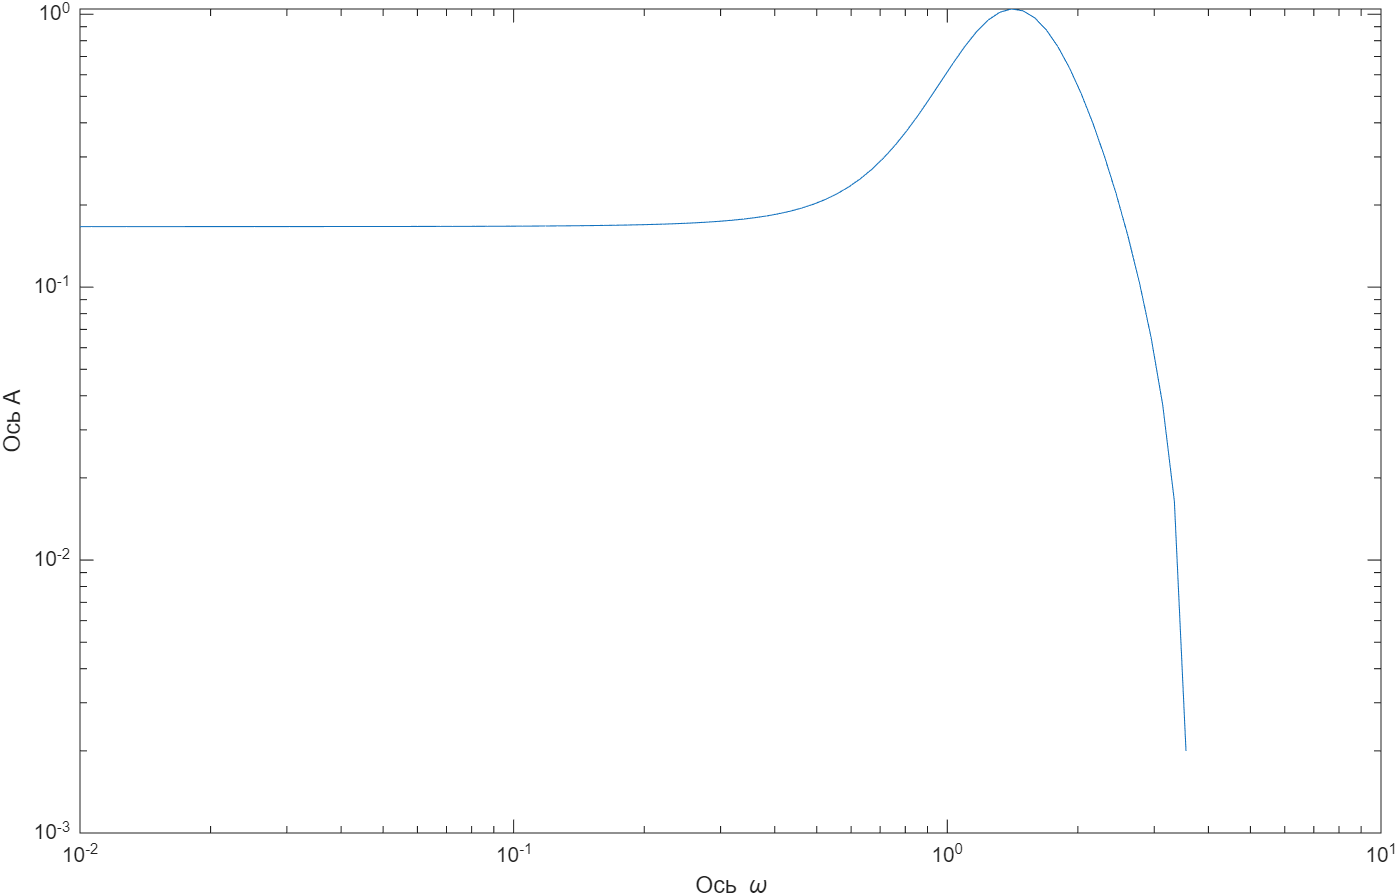
\includegraphics[width=0.75\textwidth]{figs/table_2_func_result.png}
    \caption{Результат работы table\_2\_func()}
    \label{fig:table_2_func_result.png}
\end{figure}




\subsection*{ \boxed{\text{ Задание 3. }} }
\begin{quote}
    \textit{\exThree}
\end{quote}



\begin{codemultipage}
    \captionof{listing}{Алгоритм записи результатов работы функции в файл\label{lst:write_results.m}}
    \inputminted{matlab}{code/write_results.m}
\end{codemultipage}


Данный алгоритм записывает результаты работы функции из задания 1 в файл в следующем виде, где на строках 2--9 представлены значения осей $x_1$, $x_2$ и $y$ соответственно:

\begin{codemultipage}
    \captionof{listing}{Пример результата работы \cref{lst:write_results.m}\label{lst:example_results.txt}}
    \inputminted{x}{code/example_results.txt}
\end{codemultipage}

Реализация задания основана на особенностях функции \mintinline{x}!fprintf()! в математическом пакете MatLab.
Она заключается в следующем: если составить массив вида
$$
    data = \left[
    \begin{array}{cccc}
        x_1^1 & x_1^2 & \dots & x_1^n \\
        x_2^1 & x_2^2 & \dots & x_2^n \\
        y^1   & y^2   & \dots & y^n
    \end{array}
    \right],
$$
то вызов функции в виде \mintinline{matlab}!fprintf(output_stream, '%f %f %f\n', data)! будет записывать в файл построчно значения ($x_1^1$, $x_2^1$, $y^1$), затем ($x_1^2$, $x_2^2$, $y^2$) и т.д. Данная особенность работы \mintinline{x}!fprintf()! позволяет избежать использование цикла для записи значений в файл.

Опишем процесс выражения векторов $x_1$, $x_2$ и $y$ в виде матрицы $data$.
Поскольку $x_1$ и $x_2$ являются результатами работы функции \mintinline{x}!meshgrid()! (см. \cref{lst:table_1_func.m}), они имеют вид матриц размера $m \times n$, где $m$ и $n$ --- количество точек по соответствующим осям.
Вектор $y$ имеет те же размеры, т.к. является результатом вычислений над матрицами $x_1$ и $x_2$.

Для того, чтобы представить все три матрицы в виде вектор-строк необходимо использовать конструкцию вида \mintinline{x}!x(:)'!.
Для начала мы превращаем матрицу $m \times n$ в вектор-столбец размера $mn \times 1$, используя \mintinline{x}!(:)! (благодаря особенности работы MatLab), затем транспонируем его в вектор-строку $1 \times mn$, используя апостроф \mintinline{x}!'!.

Таким образом мы получаем вектор-строку $x$.
Используем данный синтаксис для всех трёх матриц и объединяем полученные вектор-строки в матрицу $data$ размера $3 \times mn$.


\subsection*{ \boxed{\text{ Задание 4. }} }
\begin{quote}
    \textit{\exFour}
\end{quote}

\begin{codemultipage}
    \captionof{listing}{Алгоритм обработки изображений\label{lst:image_ex.m}}
    \inputminted{matlab}{code/image_ex.m}
\end{codemultipage}

Для выполнения первой подзадачи следует получить границы каждой из 4${}^\underline{\text{х}}$ частей изображения (см. строки 15--15).
Обозначим разделенные части изображения по сторонам света, где NW --- северо запад, NE --- северо восток, SW --- юго запад, SE --- юго восток.
Получение четвертей изображения возможно благодаря срезам исходного.
Особенность хранения изображений в MatLab заключается в том, что они хранятся в виде трёхмерных массивов, которые можно вообразить так: матрица имеет вид трёх, лежащих друг на друге, листов бумаги, где каждый лист соответствует одному из цветовых каналов RGB (первый канал --- красный (R), второй --- зеленый (G), третий -- синий (B)), а вместо клеток на листочках --- координаты пикселей.
Таким образом, для получения NW части изображения необходимо взять срезы по строкам от 1 до \mintinline{x}!half_rows! и по столбцам от 1 до \mintinline{x}!half_cols!.
Аналогично для остальных частей изображения.

Для выполнения второй подзадачи необходимо применить к каждой из частей изображения соответствующую операцию.
Для NW части --- зеркальное отображение, для NE --- полный разворот, для SW --- инверсия цвета, для SE --- замена одного цвета на другой.

\begin{enumerate}
    \item Первая подзадача реализована встроенной функцией \mintinline{x}!flip(..., 2)!, где в качестве второго аргумента дано число $2$, обозначающее направление, относительно которого будет происходить отражение (в данном случае по строкам): $\left[1~~2~~3\right] \rightarrow \left[ 3~~2~~1 \right]$.
    \item Вторая подзадача так же реализована с помощью встроенной функции \mintinline{x}!rot90(..., 2)!, где второй аргумент $2$ обозначает количество поворотов на $90^\circ$ по часовой стрелке.
    \item Треться подзадача так же не требует дополнительных пояснений, т.к. существует встроенная для данной операции функция \mintinline{x}!imcomplement! (которая просто вычитает значения пикселей из $255$, тем самым добиваясь инверсии).
    \item Четвертая подзадача заключается в замене одного цвета на другой. В качестве цели замены выбран черный цвет пиджаков. На строке 49 задается примерный оттенок черного цвета, а в строке 50 --- погрешность. Таким образом будут заменяться все оттенки в диапазоне $0 \div 30$. На строках 51--54 создается маска, которая будет принимать значения логической 1 в пикселях, подходящим заданным условиям (оттенок $0 \div 30$). Затем, на строках 57--59 происходит замена цвета в подходящих пикселях по трем цветовым каналам RGB. Поскольку было решено заменить цвет пиджаков на ярко красный, то зеленые и синии каналы следует заглушить до нуля путем поэлементного умножения на логически инвертированную маску (т.к. подходящие пиксели в маске имеют значение 1, а не подходящие --- 0, то инвертирование даст нам возможность обнулить нужные пиксели). Красный канал, наоборот, необходимо увеличить до максимума (255) в подходящих пикселях, что достигается путем предварительного заглушения, а затем прибавления значения 255.
\end{enumerate}

Результат работы алгоритма \cref{lst:image_ex.m} представлен на рисунках ниже.

\begin{figure}[H]
    \centering
    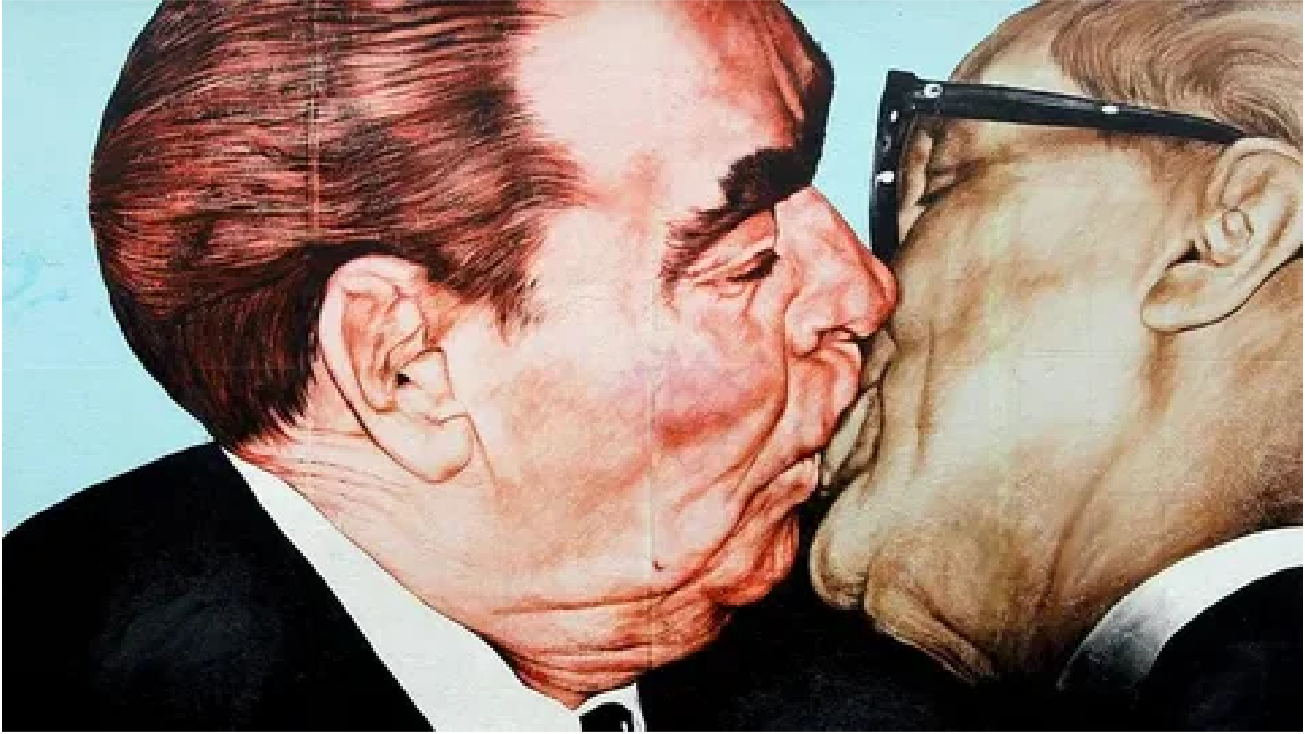
\includegraphics[width=0.7\textwidth]{figs/bre.png}
    \caption{Исходное изображение}
    \label{fig:bre.png}
\end{figure}

\begin{figure}[H]
    \centering
    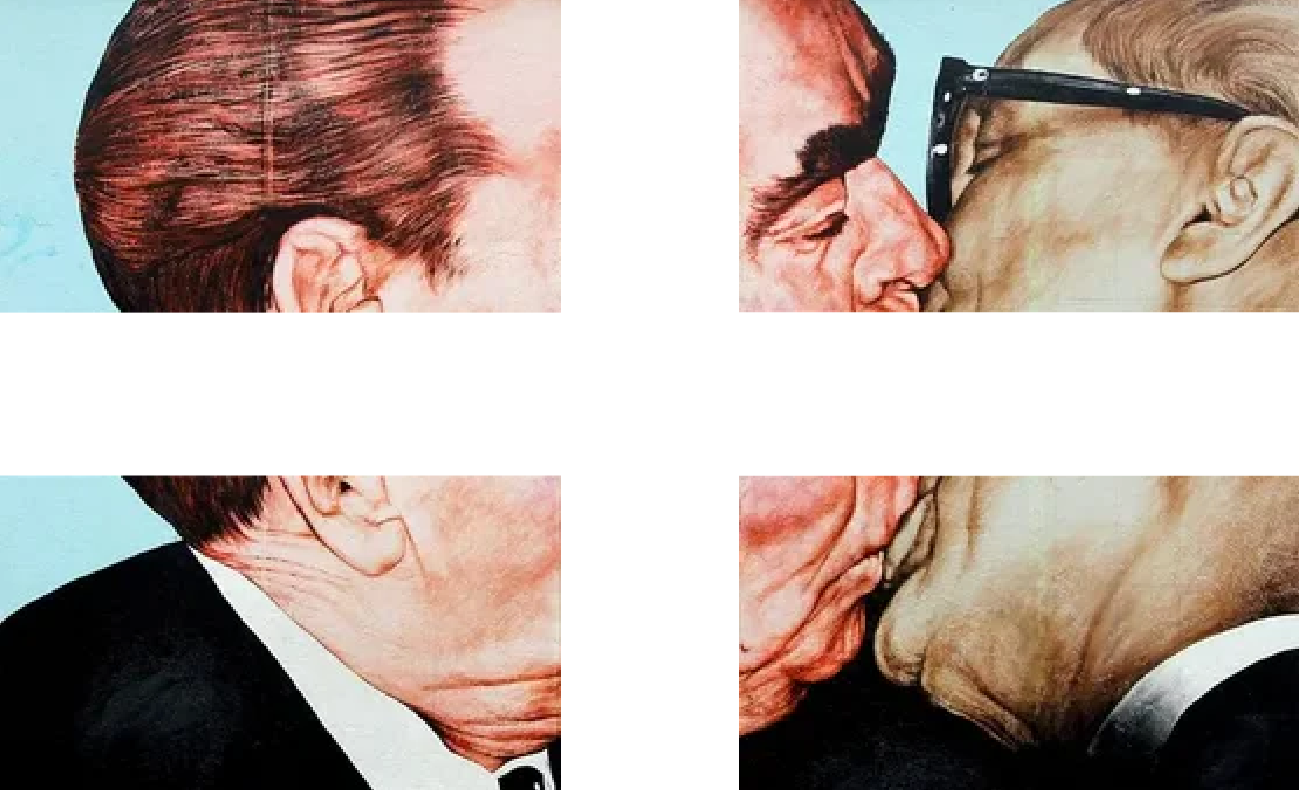
\includegraphics[width=0.7\textwidth]{figs/parted.png}
    \caption{Разделенное изображение}
    \label{fig:parted.png}
\end{figure}

\begin{figure}[H]
    \centering
    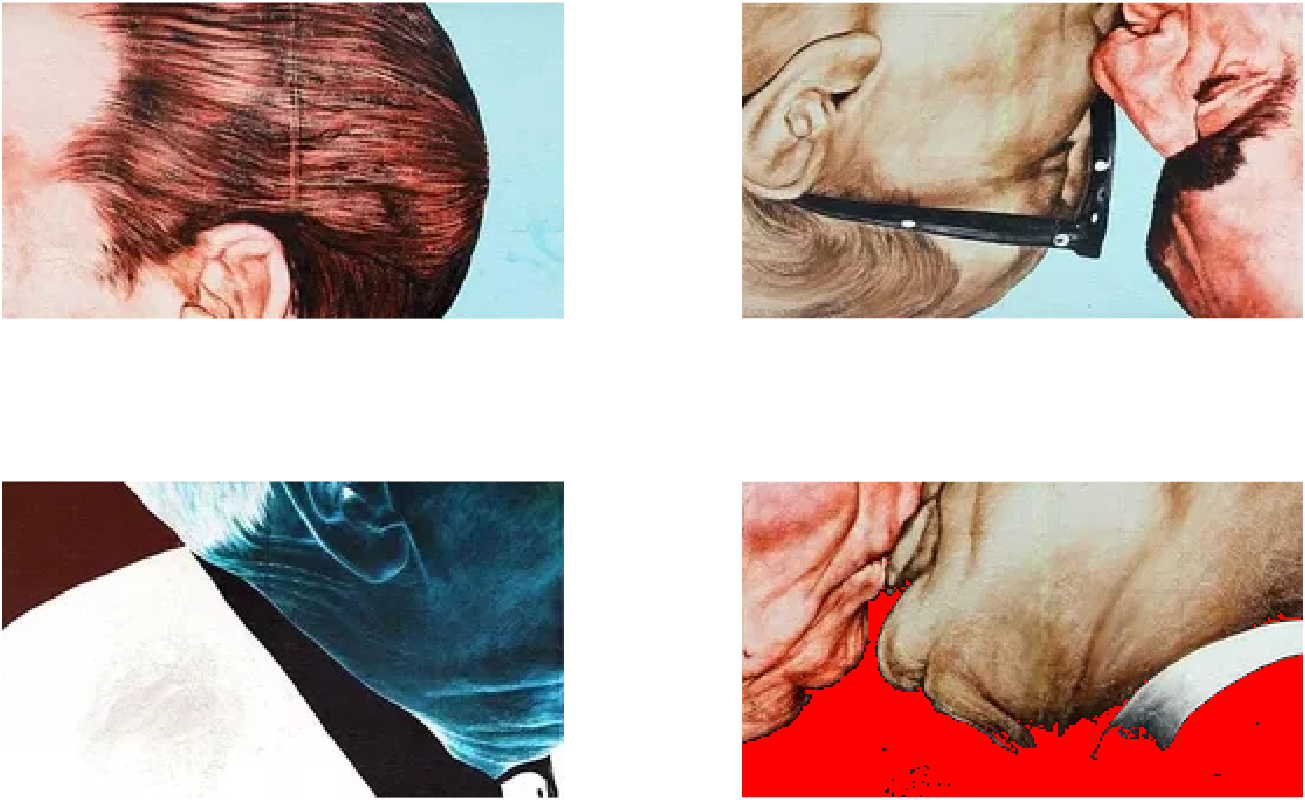
\includegraphics[width=0.7\textwidth]{figs/processed.png}
    \caption{Обработанные изображения}
    \label{fig:processed.png}
\end{figure}






\section*{Выводы.}
Алгоритмы и функции работают исправно и корректно выполняют поставленные задачи.

Были решены все задачи. Цель лабораторной работы была успешно достигнута, продемонстрировав владение всеми необходимыми знаниями для работы с функциями и файлами в математическом пакете MatLab.

% \begin{figure}[hbt]
%     \centering
%     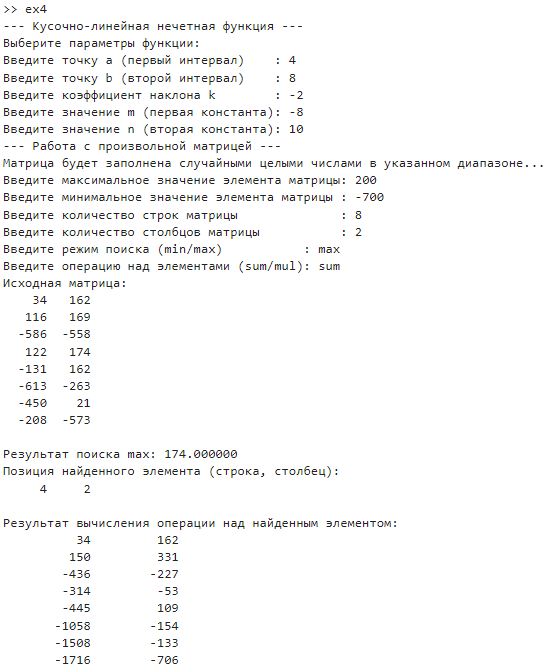
\includegraphics[width=\linewidth, height=0.75\textheight, keepaspectratio]{figs/result.png}
%     \caption{Вызов программы}
%     \label{fig:result.png}
% \end{figure}

% \begin{figure}[hbt]
%     \centering
%     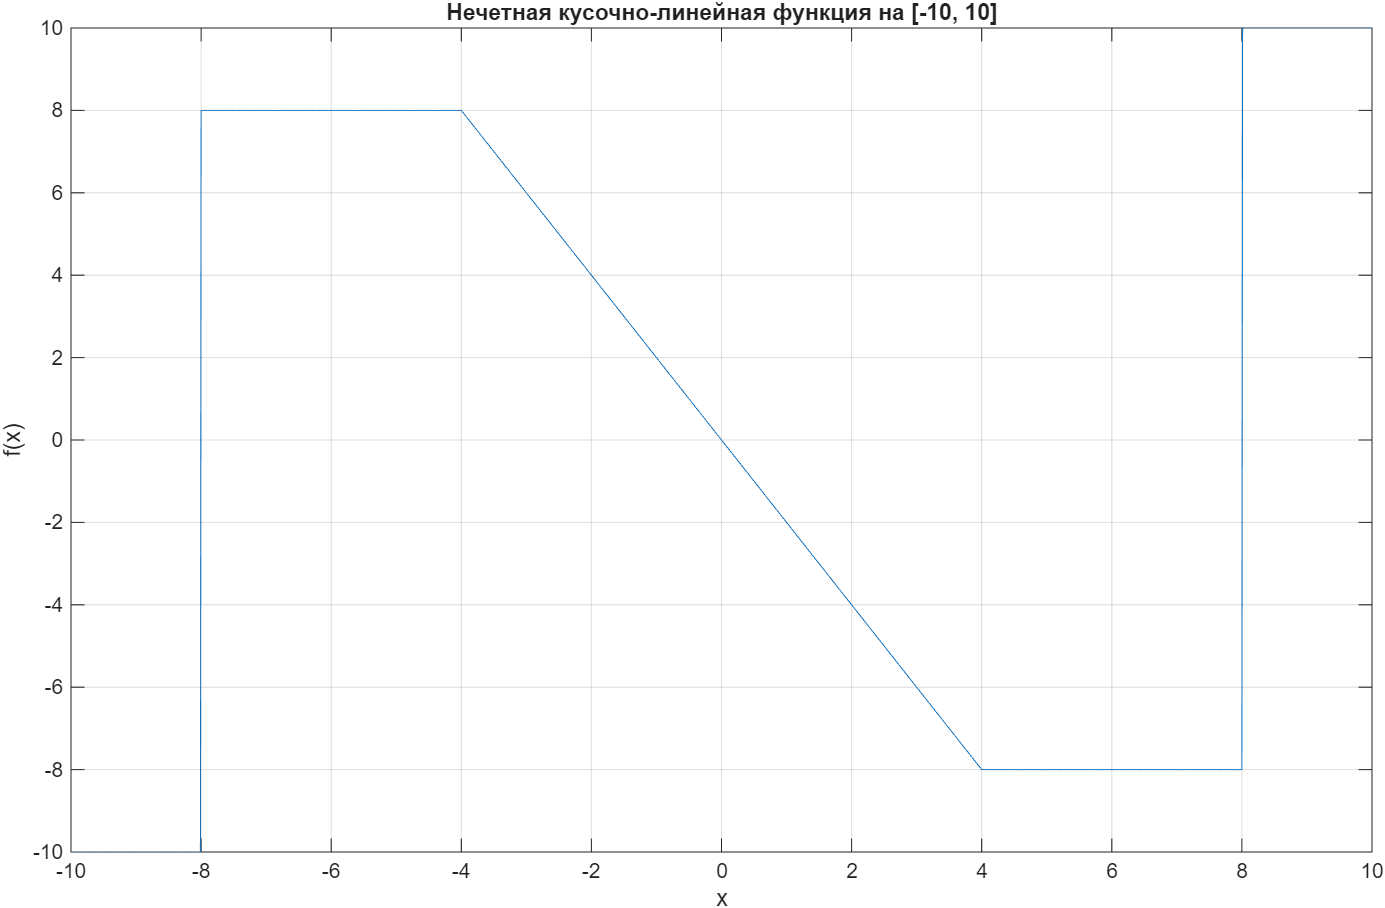
\includegraphics[width=1.00\textwidth]{figs/result_figure.png}
%     \caption{График при параметрах из \cref{fig:result.png}}
%     \label{fig:result_figure.png}
% \end{figure}

